\section{从概率论走向随机微积分：先补齐语言}
\label{bg:sec:language}

本节先用 $X$ 泛指一般随机过程；进入金融模型后，$S$ 专指价格，$X=\log S$ 专指对数价格。
题目中的 $W_t$、$\mathrm dW_t$ 和 $\mathrm dX_t$ 看起来都带着微积分符号，
但不能直接按普通导数运算。本节从已经熟悉的随机变量出发，说明这些符号究竟代表什么。
学习时先抓住三个问题：\emph{随机性在哪里？在时刻 $t$ 已经知道什么？一个很短时间段中的变化有多大？}
这三个问题贯穿后面的公式推导和程序实现。

\subsection{随机变量是一张照片，随机过程是一段随机影片}
\label{bg:sub:process}

一个随机变量 $Y$ 给每个可能的实验结果 $\omega$ 指定一个数 $Y(\omega)$。
随机过程则是一族带时间下标的随机变量 $\{X_t:t\geq 0\}$。
这里有两种不同的观察方式：固定时间 $t$，$X_t$ 是一个随机变量，可以讨论其均值、方差和分布；
固定一次实验结果 $\omega$，映射 $t\mapsto X_t(\omega)$ 是一条\emph{样本路径}。
模拟一次完整实验，得到一条路径；重新抽取随机数，通常会得到另一条路径。

例如，用 $S_t$ 表示时刻 $t$ 的资产价格。$S_1$ 表示一年后的随机价格，
而整条 $\{S_t:0\leq t\leq 1\}$ 还记录这一年中价格经过了哪些位置。
终点分布相同的两个模型，中途波动方式可能很不一样。
这也解释了为什么“比较终点平均价格”和“逐条比较两种模拟得到的路径”是两件不同的事。

在计算机中，连续时间通常被离散成一个网格。若总时长为 $T$，分成 $N$ 步，则
\begin{equation}
  h=\frac{T}{N},\qquad t_n=nh,\qquad n=0,1,\ldots,N.
  \label{bg:eq:grid}
\end{equation}
一条离散路径就是长度为 $N+1$ 的数列 $(X_0,X_1,\ldots,X_N)$，
其中程序中的 $X_n$ 通常代表连续过程在 $t_n$ 附近的近似值。
网格越密意味着时间分辨率越高；增加模拟路径数则是重复更多次随机实验。
这两个操作改变的是不同的量。

还要区分随机变量与随机变量的一次数值实现。表达式 $\E[X_T]$ 是模型分布决定的一个数；
某次模拟的终点 $X_T(\omega)$ 只是一个观测值，不会因为计算正确就恰好等于该均值。
把很多条路径在同一时刻取平均，可以观察平均行为；把同一条路径在很多时刻取平均，
得到的则是另一个统计量。两种平均不能在没有依据时互换。

\subsection{普通微分方程为什么可以改写成积分方程}
\label{bg:sub:ode}

先暂时去掉随机性。普通微分方程
\begin{equation}
  \frac{\mathrm dx(t)}{\mathrm dt}=a(t,x(t)),\qquad x(0)=x_0
  \quad\Longleftrightarrow\quad
  x(t)=x_0+\int_0^t a(s,x(s))\,\mathrm ds
  \label{bg:eq:ode}
\end{equation}
表示当前位置等于初始位置加上从开始到现在的累计变化。
例如 $a(t,x)=rx$ 表示瞬时增长速度与当前数量成正比。
在一个短时间段内把增长速度暂时冻结在左端，就得到
\begin{equation}
  x(t_{n+1})-x(t_n)\approx a(t_n,x(t_n))h.
  \label{bg:eq:ode-euler}
\end{equation}
这是普通 Euler 方法的来源。
随机微分方程也将采用“初值加累计变化”的表达方式，
只是累计变化中多出一种随机积分。因此，理解随机积分比寻找 $W_t$ 的普通导数更重要。

\section{布朗运动：把连续时间的随机冲击建模}
\label{bg:sec:brownian}

\subsection{定义与最需要记住的尺度}
\label{bg:sub:brownian-definition}

标准布朗运动 $W=\{W_t:t\geq0\}$ 满足：$W_0=0$；样本路径几乎必然连续；
不相交时间区间上的增量相互独立；并且对 $0\leq s<t$，
\begin{equation}
  W_t-W_s\sim\mathcal N(0,t-s).
  \label{bg:eq:brownian-increment}
\end{equation}
记号 $\mathcal N(m,v)$ 的第二个参数是\emph{方差}。
特别地，长度为 $h$ 的时间段中的增量可以写成
\begin{equation}
  \Delta W_n=W_{t_{n+1}}-W_{t_n}=\sqrt h\,Z_n,
  \qquad Z_n\sim\mathcal N(0,1),
  \label{bg:eq:normal-scaling}
\end{equation}
其中不同时间段使用独立的 $Z_n$。于是
\begin{equation}
  \E[\Delta W_n]=0,\qquad
  \Var(\Delta W_n)=h,\qquad
  \operatorname{sd}(\Delta W_n)=\sqrt h.
  \label{bg:eq:increment-moments}
\end{equation}

独立的是不相交时间段的\emph{增量}，不是不同时间的布朗运动取值。
例如 $W_t$ 包含此前的 $W_s$，所以它们共享历史波动。对 $s\leq t$，
\begin{equation}
  \Cov(W_s,W_t)=\E[W_s(W_s+W_t-W_s)]=s,
  \label{bg:eq:brownian-covariance}
\end{equation}
其中交叉项因独立且零均值而为零。
如果在每个时间点分别抽取一个独立的 $\mathcal N(0,t)$ 变量，虽然每个时点的边际分布正确，
时间点之间的关系却错了，因而不会得到布朗路径。正确做法是生成独立增量，再累计成取值。

\textbf{随机增量的典型大小是 $\sqrt h$，不是 $h$。}
“典型大小”在这里可由标准差衡量，不能理解为每一次增量都等于 $\sqrt h$。
例如 $h=0.01$ 时，单位布朗运动的增量标准差为 $0.1$。
如果误写成 $hZ_n$，$N=T/h$ 步累计增量的方差将是 $Nh^2=Th$，
随着网格加密趋于零；正确写成 $\sqrt h Z_n$，累计方差则为 $Nh=T$。
前一种写法会在极限中把随机波动抹掉。

比较 $h$ 与 $\sqrt h$ 还有一个容易误解的地方：在足够短的时间段里，
非零扩散项的典型幅度可能比漂移项大，但这不表示漂移在整个时间区间内不重要。
连续 $N$ 步的同向确定性变化按 $Nh$ 累积，独立零均值随机冲击则通过方差按 $Nh$ 累积，
其标准差按 $\sqrt{Nh}$ 衡量。局部尺度的比较与长时间累计效果的比较，需要分别进行。

虽然路径连续，布朗运动却不是一条光滑曲线。
例如在固定时刻观察短区间的差商，有
\begin{equation}
  \frac{W_{t+h}-W_t}{h}\sim\mathcal N\!\left(0,\frac1h\right).
  \label{bg:eq:brownian-difference-quotient}
\end{equation}
它的尺度随 $h\downarrow0$ 而增大，已经提示普通导数的直觉不适用。
更强的结论是布朗样本路径几乎必然处处不可微；这里只把它作为背景事实，
不把差商的分布计算冒充这一结论的完整证明。
因此，$\mathrm dW_t/\mathrm dt$ 不能当作一个普通函数代入常微分方程。

\begin{figure}[htbp]\centering
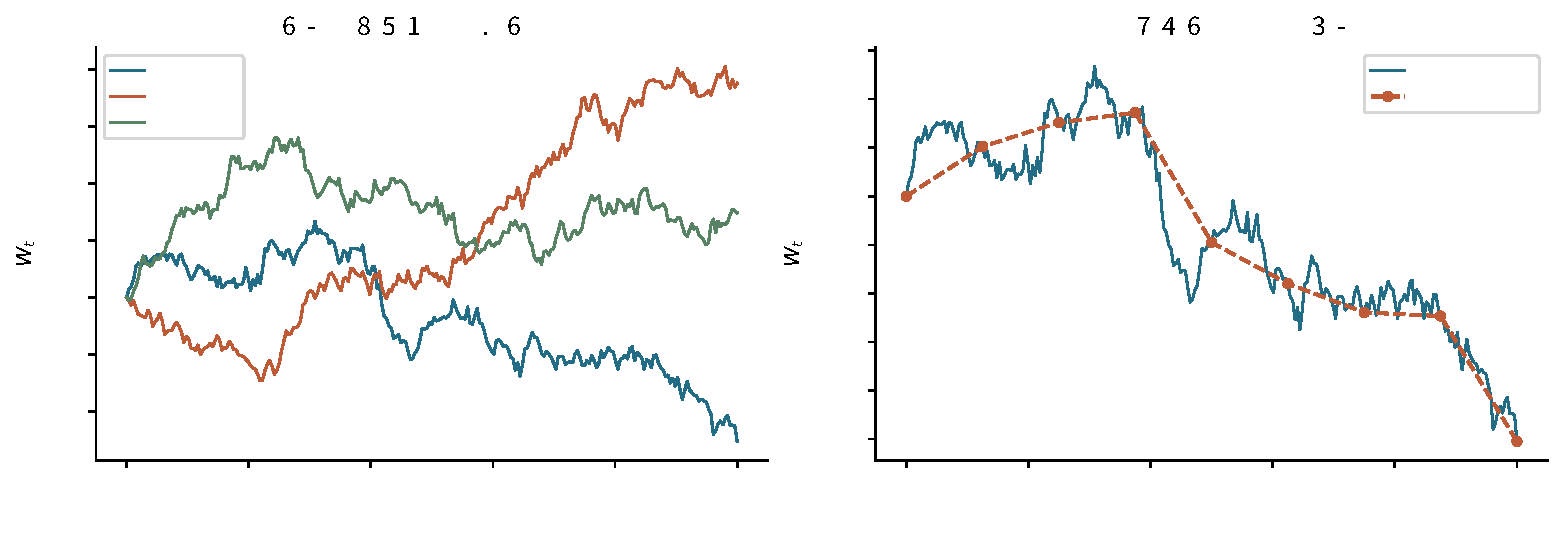
\includegraphics[width=\textwidth]{assets/brownian_coupling.pdf}
\caption{左图展示同一布朗模型的不同样本路径；右图展示同一路径的粗细网格取值。细网格之间也用直线连接以便展示，折线不是连续布朗运动的完整轨迹。}\label{fig:bg-brownian}
\end{figure}
图~\ref{fig:bg-brownian} 右图中，粗网格在共同时间点与细网格完全一致，因为每个粗增量来自相邻细增量求和。后面的强收敛实验正要使用这种设计。

\subsection{用随机游走理解布朗运动的来源}
\label{bg:sub:random-walk}

可以想象每隔 $h$ 秒抛一次公平硬币，向上或向下走 $\sqrt h$：
\begin{equation}
  R_{kh}^{(h)}=\sqrt h\sum_{j=1}^k\xi_j,
  \qquad
  \Pr(\xi_j=1)=\Pr(\xi_j=-1)=\frac12,
  \label{bg:eq:random-walk}
\end{equation}
其中 $\xi_j$ 独立。走过时间 $kh$ 后，均值为零，方差为 $kh$。
当 $h$ 变小，同一段时间内包含越来越多的小冲击。
中心极限定理解释了为什么在固定时间观察时，累计位移接近正态分布；
独立投掷也保留了不相交区间增量的独立性。
进一步的过程极限定理能够把适当插值后的整条随机游走与布朗运动联系起来，
但该结论比单个随机变量的中心极限定理更强，本讲义不证明它。

数值计算不必真的抛硬币。利用式\eqref{bg:eq:normal-scaling}直接生成独立正态增量，
就能\emph{精确生成布朗运动在所选网格上的联合分布}。
这并不意味着已精确得到某个随机微分方程的解；从布朗增量更新状态的公式，仍可能产生离散误差。

\section{信息、条件期望与鞅：为什么不能偷看未来}
\label{bg:sec:information}

\subsection{把“截至现在知道的一切”记作 $\mathcal F_t$}
\label{bg:sub:filtration}

用 $\mathcal F_t$ 表示截至时刻 $t$ 已经掌握的信息。
严格说，它是由事件组成的 $\sigma$-代数；直观上，可以先把它看成截至 $t$ 的完整观测记录。
随着时间推移，记录只会增加，因此当 $s\leq t$ 时，$\mathcal F_s\subseteq\mathcal F_t$。
这样一族逐渐增加的信息称为\emph{滤过}。
对于布朗运动，可以使用它自身的历史信息，也可以再加入与未来增量独立的初始信息。
所选滤过必须使未来的布朗增量仍独立于当前信息。

过程 $H_t$ 是\emph{适应的}，意思是 $H_t$ 可以由时刻 $t$ 已有的信息确定。
例如 $H_t=W_t$、$H_t=\max_{0\leq s\leq t}W_s$ 可以在当时算出；
而 $H_t=W_{t+1}$ 需要提前知道未来，通常不适应。
在模拟中，适应性对应一个非常具体的顺序：先用当前状态确定系数，再抽取下一步的新冲击。

\subsection{条件期望是根据已有信息作平均预测}
\label{bg:sub:martingale}

$\E[Y\mid\mathcal F_s]$ 表示已知时刻 $s$ 信息后，对未来量 $Y$ 的平均预测。
因为 $W_t=W_s+(W_t-W_s)$，而未来增量独立于过去且均值为零，
\begin{equation}
  \E[W_t\mid\mathcal F_s]=W_s,
  \qquad 0\leq s\leq t.
  \label{bg:eq:w-martingale}
\end{equation}
一般地，可积、适应的过程 $M_t$ 若满足
\begin{equation}
  \E[M_t\mid\mathcal F_s]=M_s,
  \qquad 0\leq s\leq t,
  \label{bg:eq:martingale-definition}
\end{equation}
就称为\emph{鞅}。直观含义是：给定全部过去信息，未来的平均值等于当前值。
这并不表示每条路径保持不变，也不表示未来不可能大幅上升或下降。

条件期望还给出
\begin{equation}
  \E[W_t^2\mid\mathcal F_s]=W_s^2+(t-s),
  \qquad
  \E[W_t^2-t\mid\mathcal F_s]=W_s^2-s.
  \label{bg:eq:w-square-martingale}
\end{equation}
所以 $W_t^2$ 的平均值在增长，而 $W_t^2-t$ 是鞅。
这里减去的时间项 $t$ 不是人为技巧；它正是后面 It\^o 公式中额外修正项的来源。

可以把条件期望理解成先暂停影片，再对后续的所有可能分支取平均。
例如在时刻 $1$ 已经观察到 $W_1=w$，那么 $W_2=w+Z$，其中新的 $Z\sim\mathcal N(0,1)$。
未来值的条件均值是 $w$，条件二阶矩是 $w^2+1$。
暂停时看到的 $w$ 是已知量；尚未发生的 $Z$ 才是这次条件平均中保留的随机性。
这与一开始尚未看到任何路径时直接求 $\E[W_2]=0$ 并不矛盾。

\section{It\^o 积分：按时间累计随机冲击}
\label{bg:sec:ito-integral}

\subsection{先在有限网格上定义，再取极限}
\label{bg:sub:left-sum}

普通积分 $\int_0^T H_s\,\mathrm ds$ 是把许多 $H\times$ 时间长度加起来。
随机积分 $\int_0^T H_s\,\mathrm dW_s$ 则把许多 $H\times$ 布朗增量加起来。
先考虑分段常数过程：在 $[t_i,t_{i+1})$ 上取 $H_s=H_i$，且 $H_i$ 只依赖 $\mathcal F_{t_i}$。
定义
\begin{equation}
  I_T=\int_0^T H_s\,\mathrm dW_s
  :=\sum_{i=0}^{N-1}H_i(W_{t_{i+1}}-W_{t_i}).
  \label{bg:eq:ito-simple-definition}
\end{equation}
这就是 It\^o 积分的基本构件。左端信息的选择很关键：在下一段冲击出现之前，$H_i$ 已经确定。
即使 $H_i$ 是随机的，它也没有利用这一段尚未发生的增量。

对更一般的被积过程，先用这类简单过程逼近，再把积分定义为均方意义下的极限。
本讲义使用一个方便的充分条件：$H$ 有适当的时间可测性（例如连续且适应），并满足
\begin{equation}
  \E\!\left[\int_0^T H_s^2\,\mathrm ds\right]<\infty.
  \label{bg:eq:ito-square-integrable}
\end{equation}
“均方收敛”指 $\E[|I^{(n)}-I|^2]\to0$。
这里并非要求对每条布朗路径做普通 Riemann--Stieltjes 积分，
也不能对任意粗糙的 $H$ 不加条件地声称所有左端求和都收敛。
连续、适应且具有适当矩控制的情形，足以覆盖后面大部分直观推导。

\subsection{两个核心性质：均值为零，方差可以计算}
\label{bg:sub:isometry}

因为 $H_i$ 在 $t_i$ 已知，利用条件期望有
\begin{equation}
  \E[H_i\Delta W_i]
  =\E\!\left[H_i\E[\Delta W_i\mid\mathcal F_{t_i}]\right]=0.
  \label{bg:eq:zero-mean-step}
\end{equation}
不同时间段的加权增量不一定相互独立，但它们的交叉项期望为零。
例如 $i<j$ 时，$H_i\Delta W_i H_j$ 在 $t_j$ 已知，再对 $\Delta W_j$ 取条件期望即可。
展开式\eqref{bg:eq:ito-simple-definition}的平方，因此得到
\begin{align}
  \E[I_T]&=0,\label{bg:eq:ito-mean}\\
  \E[I_T^2]
  &=\sum_{i=0}^{N-1}\E[H_i^2](t_{i+1}-t_i)
   =\E\!\left[\int_0^T H_s^2\,\mathrm ds\right].
  \label{bg:eq:ito-isometry}
\end{align}
式\eqref{bg:eq:ito-isometry}称为\emph{It\^o 等距公式}。
通过均方极限，两条性质推广到满足式\eqref{bg:eq:ito-square-integrable}的过程。
特别地，此时 $\int_0^t H_s\,\mathrm dW_s$ 是均值为零的平方可积鞅。

例如当 $H_s=c$ 是常数时，积分等于 $cW_T$，其方差为 $c^2T$。
当 $H_s$ 本身也随机时，等距公式仍可计算二阶矩，却\emph{不能据此断言积分一定服从正态分布}。
后面的 $\int_0^T W_s\,\mathrm dW_s$ 就是反例。
还应记住：“随机积分的期望是零”需要可积性条件。
后面若要对一个 SDE 两边取期望，必须先确认随机积分满足相应条件，不能只看见 $\mathrm dW$ 就把它删掉。

作为等距公式的另一例，取确定性被积函数 $H_s=s$，便有
\begin{equation}
  \E\!\left[\int_0^T s\,\mathrm dW_s\right]=0,
  \Var\!\left(\int_0^T s\,\mathrm dW_s\right)
  =\int_0^T s^2\,\mathrm ds=\frac{T^3}{3}.
  \label{bg:eq:deterministic-integrand}
\end{equation}
后半段的冲击被赋予更大的权重，因此总波动也取决于权重的平方。
这里被积函数是确定的，有限求和均为独立正态变量的线性组合，极限仍为正态变量。
这项额外的分布结论依赖确定性权重，不能从等距公式本身推出。

\section{二次变差：为什么随机微积分多出一项}
\label{bg:sec:quadratic-variation}

\subsection{小增量平方后，累计起来并不消失}
\label{bg:sub:qv-calculation}

在均匀网格上定义布朗增量的平方和
\begin{equation}
  Q_N=\sum_{i=0}^{N-1}(\Delta W_i)^2,
  \qquad h=T/N.
  \label{bg:eq:qv-sum}
\end{equation}
由 $\Delta W_i=\sqrt h Z_i$，以及标准正态变量的矩
$\E[Z_i^2]=1$、$\E[Z_i^4]=3$，可得
\begin{align}
  \E[Q_N]&=Nh=T,\label{bg:eq:qv-mean}\\
  \Var(Q_N)&=N\Var(hZ_i^2)
   =Nh^2(3-1)=2Th.\label{bg:eq:qv-variance}
\end{align}
于是
\begin{equation}
  \E[(Q_N-T)^2]=2Th\longrightarrow0.
  \label{bg:eq:qv-limit}
\end{equation}
这严格证明了沿这些确定性均匀网格，$Q_N$ 在 $L^2$（即均方）意义下收敛到 $T$，
从而也依概率收敛。这就是布朗运动二次变差为时间的基本计算。
对任意确定性分割，方差为 $2\sum_i(t_{i+1}-t_i)^2$，
至多是 $2T$ 乘以最大步长，因此最大步长趋于零时仍有相同的均方结论。

这里的收敛可以用熟悉的概率不等式解释：由 Chebyshev 不等式，
对任意固定的 $\varepsilon>0$，$\Pr(|Q_N-T|>\varepsilon)\leq 2Th/\varepsilon^2$。
所以网格越细，平方和偏离 $T$ 超过指定容忍量的概率越小。
这与声称“所有网格、所有路径上都精确等于 $T$”有本质区别。

与之对照，时间增量平方和为 $\sum_i h^2=Th\to0$。
布朗增量和时间增量的混合项也较小，例如
\begin{equation}
  \E\!\left[\sum_{i=0}^{N-1}|h\Delta W_i|\right]
  =T\sqrt{\frac{2h}{\pi}}\longrightarrow0.
  \label{bg:eq:mixed-increment}
\end{equation}
因此，普通微积分里通常丢掉的二阶小量中，
$(\Delta W)^2$ 在累计后却能留下一个非零极限。

\subsection{$(\mathrm dW_t)^2=\mathrm dt$ 是积分计算的记账规则}
\label{bg:sub:ito-table}

以上结论常被压缩成下表，便于展开二阶项：
\begin{center}
\begin{tabular}{lll}
\toprule
形式乘积 & 累计后的有效项 & 原因\\
\midrule
$\mathrm dt\,\mathrm dt$ & $0$ & 时间增量平方和趋于零\\
$\mathrm dt\,\mathrm dW_t$ & $0$ & 混合增量求和趋于零\\
$\mathrm dW_t\,\mathrm dW_t$ & $\mathrm dt$ & 布朗增量平方和趋于时间\\
\bottomrule
\end{tabular}
\end{center}
这是一套与极限相联系的记账规则，\emph{不是普通无穷小实数之间的代数恒等式}。
尤其不能说每一步都有 $(\Delta W_i)^2=h$：事实上
$(\Delta W_i)^2/h=Z_i^2$，其方差始终为 $2$，并不因为 $h$ 变小就集中到 $1$。
真正接近确定数的是许多平方增量的\emph{累计结果}。

推导 It\^o 公式时还会遇到带权平方和。
如果权重 $K_i$ 在 $t_i$ 已知且 $|K_i|\leq C$，条件期望和交叉项正交给出
\begin{equation}
  \E\!\left[\left(\sum_i K_i\big((\Delta W_i)^2-h\big)\right)^2\right]
  \leq 2C^2Th\longrightarrow0.
  \label{bg:eq:weighted-qv}
\end{equation}
这说明把二阶 Taylor 展开中的平方增量替换为时间增量，也有极限依据。
对于无界系数，需要进一步的可积性估计或先在有界区域内处理，不能无条件照搬这个界。

\section{从 Taylor 展开理解 It\^o 公式}
\label{bg:sec:ito-formula}

\subsection{先看 $f(t,W_t)$}
\label{bg:sub:ito-taylor}

设 $f(t,x)$ 对时间有一阶连续偏导、对空间有二阶连续偏导。
符号 $f_t,f_x,f_{xx}$ 分别表示这些偏导数。
为理解公式，先想象 $f$ 足够光滑，而且需要的导数在所研究区域内有界。
在一个很短的时间段，对函数增量作二阶 Taylor 展开，主要项是
\begin{equation}
  f(t+h,W_t+\Delta W)-f(t,W_t)
  \approx f_t h+f_x\Delta W+\frac12 f_{xx}(\Delta W)^2,
  \label{bg:eq:taylor-brownian}
\end{equation}
右侧偏导均在左端 $(t,W_t)$ 处计算。
含 $h^2$、$h\Delta W$ 的项求和后消失；含 $(\Delta W)^2$ 的项不能忽略。
把这些增量沿网格加起来并取极限，就得到
\begin{align}
  f(T,W_T)-f(0,W_0)
  &=\int_0^T\left(f_t(s,W_s)+\frac12 f_{xx}(s,W_s)\right)\,\mathrm ds
  \notag\\
  &\quad+\int_0^T f_x(s,W_s)\,\mathrm dW_s.
  \label{bg:eq:ito-brownian-integral}
\end{align}
其微分写法为
\begin{equation}
  \mathrm df(t,W_t)
  =\left(f_t+\frac12f_{xx}\right)\mathrm dt+f_x\,\mathrm dW_t.
  \label{bg:eq:ito-brownian-differential}
\end{equation}
额外出现的 $\frac12 f_{xx}\,\mathrm dt$ 称为 It\^o 修正项。
函数有曲率时，零均值随机扰动的正负效应经过非线性变换后通常不能抵消。
例如平方函数向上弯，正负偏移都会增加平方的平均值。

这段推导解释了各项的来源，但并非对一般 $C^{1,2}$ 函数的完整证明。
严格证明还需要控制余项、证明随机积分和带权二次变差的收敛，并在需要时作局部化处理。
本讲义后续使用的是这些条件下成立的 It\^o 公式本身。

\subsection{关键例子：$\int_0^T W_s\,\mathrm dW_s$}
\label{bg:sub:w-dw}

取 $f(x)=x^2$，则 $f_x=2x$、$f_{xx}=2$，由式\eqref{bg:eq:ito-brownian-differential}得到
\begin{equation}
  \mathrm d(W_t^2)=2W_t\,\mathrm dW_t+\mathrm dt,
  \qquad
  \int_0^T W_s\,\mathrm dW_s=\frac{W_T^2-T}{2}.
  \label{bg:eq:w-dw-example}
\end{equation}
如果机械套用普通链式法则，会漏掉 $-T/2$。
漏项后的结果均值为 $T/2$，而正确随机积分的均值应为零；这提供了一个立即可做的一致性检查。
同时，这个积分一般不服从正态分布，因为 $W_T^2$ 是正态变量的平方。

还可以完全通过有限求和看见修正项。恒等式
\begin{equation}
  W_{t_{i+1}}^2-W_{t_i}^2
  =2W_{t_i}\Delta W_i+(\Delta W_i)^2
  \label{bg:eq:square-telescoping}
\end{equation}
对 $i$ 求和后，左侧首尾相消；再用式\eqref{bg:eq:qv-limit}，就得到同一个答案。
这也说明左端取值不是装饰。
若改成右端和 $\sum_iW_{t_{i+1}}\Delta W_i$，它与左端和相差
$\sum_i(\Delta W_i)^2$，极限相差 $T$。
对布朗运动作积分，不能像对光滑路径那样认为选左端还是右端都无所谓。

\section{随机微分方程究竟在说什么}
\label{bg:sec:sde}

\subsection{SDE 的真正含义是积分等式}
\label{bg:sub:sde-meaning}

一维 It\^o 随机微分方程通常写成
\begin{equation}
  \mathrm dX_t=a(t,X_t)\,\mathrm dt+b(t,X_t)\,\mathrm dW_t,
  \qquad X_0=x_0.
  \label{bg:eq:sde-differential}
\end{equation}
它的含义是存在连续、适应的过程 $X$，满足
\begin{equation}
  X_t=x_0+\int_0^t a(s,X_s)\,\mathrm ds
             +\int_0^t b(s,X_s)\,\mathrm dW_s.
  \label{bg:eq:sde-integral}
\end{equation}
第一个积分累计普通时间变化，第二个积分累计随机冲击。
$a$ 称为\emph{漂移系数}，描述局部的平均变化趋势；$b$ 称为\emph{扩散系数}，
决定局部随机波动的大小。
将短时间内的系数冻结在左端，便得到理解和模拟都很重要的近似：
\begin{equation}
  \Delta X_n\approx a(t_n,X_{t_n})h+b(t_n,X_{t_n})\sqrt h\,Z_n.
  \label{bg:eq:sde-local-step}
\end{equation}
给定当前信息，右侧近似增量的条件均值为 $a(t_n,X_{t_n})h$，
条件方差为 $b(t_n,X_{t_n})^2h$。
当系数随状态变化时，这只是冻结系数的\emph{一步近似}，不表示真实有限时间增量必然正态。
即使漂移为正，单步变化也可能为负，因为随机冲击可朝两个方向发生。

最简单的例子是 $a(t,x)=\mu$、$b(t,x)=\sigma$ 均为常数。直接积分可得
\begin{equation}
 X_t=x_0+\mu t+\sigma W_t,\qquad
 \E[X_t]=x_0+\mu t,\qquad \Var(X_t)=\sigma^2t.
 \label{bg:eq:additive-sde}
\end{equation}
确定性直线给出均值，布朗运动在直线周围制造随机起伏。
由于系数不随时间和状态改变，式\eqref{bg:eq:sde-local-step}在这个特殊例子中正好给出精确的网格更新。
一般方程中，系数在一步之内继续随真实过程变化，冻结系数才会成为近似。
这个例子也说明扩散系数的单位与漂移不同：若状态以元、时间以年计，
漂移具有元每年的单位，扩散系数具有元每平方根年的单位，二者乘上各自的增量后才都是价格变化。

\subsection{一般的一维 It\^o 公式}
\label{bg:sub:general-ito}

对于式\eqref{bg:eq:sde-differential}，二阶 Taylor 展开中的有效平方项是
$(\mathrm dX_t)^2=b(t,X_t)^2\,\mathrm dt$。
因此，若 $f\in C^{1,2}$，则
\begin{align}
  \mathrm df(t,X_t)
  &=\left(f_t(t,X_t)+a(t,X_t)f_x(t,X_t)
          +\frac12 b(t,X_t)^2f_{xx}(t,X_t)\right)\,\mathrm dt
  \notag\\
  &\quad+b(t,X_t)f_x(t,X_t)\,\mathrm dW_t.
  \label{bg:eq:general-ito}
\end{align}
它是本题理论推导的核心工具：先选一个有用的函数 $f$，求三个偏导，再代入。
例如选 $f(x)=x^2$ 可得到二阶矩方程；选对数函数时则要求过程位于正数区域。
函数的定义域和过程是否会离开该区域，都需要单独检查。

应用时可以固定一个顺序：首先辨认原方程中的 $a$ 和 $b$；其次只对普通函数 $f(t,x)$ 求偏导；
然后把 $x$ 换回随机状态 $X_t$；最后把时间项和随机项分别合并。
求 $f_x$ 时暂时把 $x$ 当作普通实变量，完全使用熟悉的微积分。
需要新增的知识只在合成后的链式公式中：二阶空间导数会与扩散系数的平方相乘。
若 $b=0$，式\eqref{bg:eq:general-ito}便退化为普通链式法则，这也是检查公式的一个办法。

\subsection{为什么还要关心解是否存在、是否唯一}
\label{bg:sub:existence}

写出方程不自动保证它有一个合理的解。
“存在”表示确有过程满足式\eqref{bg:eq:sde-integral}；
“路径唯一”表示给定相同初值和同一条布朗运动驱动后，两个解几乎必然在所有时刻一致。
这并不表示不同随机实验会得到相同路径。

一个常用的\emph{充分条件}是：系数有合适的可测性，在所研究的有限时间区间内，
存在与 $t$ 无关的常数 $L,C$，使
\begin{align}
 |a(t,x)-a(t,y)|+|b(t,x)-b(t,y)|&\leq L|x-y|,
 \label{bg:eq:lipschitz}\\
 |a(t,x)|+|b(t,x)|&\leq C(1+|x|).
 \label{bg:eq:linear-growth}
\end{align}
若初值平方可积且与信息结构相容，这组条件保证存在唯一的强解，并有适当的二阶矩控制。
这里“强解”指在已经给定的布朗运动和概率空间上构造的解，与后面数值方法的“强收敛”不是同一个定义。

式\eqref{bg:eq:lipschitz}限制系数对状态变化的敏感程度：相近状态的变化规则不能突然差得过大。
式\eqref{bg:eq:linear-growth}限制系数增长太快，帮助防止连续方程的解在有限时间内逃向无穷大。
两式是方便使用的一组充分条件，\emph{不是必要条件}；
某些不满足它们的方程也可能有唯一解，只是需要其他论证。
它们也不保证任意数值方法自动保持真解的正性或其他性质，离散格式还须另行检查。

\subsection{进入后续推导前的自测}
\label{bg:sub:self-check}

\begin{enumerate}
  \item 时间步长从 $h$ 缩为 $h/4$ 时，布朗增量的标准差变为多少？
  \item $\E[\Delta W]=0$ 是否意味着一次模拟中的 $\Delta W=0$？
  \item 为什么不能把每一步 $(\Delta W)^2$ 都替换成 $h$ 后称为精确模拟？
  \item 若 $\mathrm dX_t=a_t\,\mathrm dt+b_t\,\mathrm dW_t$，$\mathrm d(X_t^2)$ 等于什么？
  \item 两种算法要在同一随机冲击下比较，下一步应使用同一个还是不同的 $Z_n$？
\end{enumerate}

答案依次是：标准差减半；不能，零均值描述重复实验的平均；
单步平方仍然随机，只有适当累计后的误差趋于零；
$\mathrm d(X_t^2)=(2X_ta_t+b_t^2)\,\mathrm dt+2X_tb_t\,\mathrm dW_t$；
应使用同一个 $Z_n$，这样比较的才是在相同驱动下两种更新规则的差异。
如果这些答案及其理由已经清楚，便具备阅读本题精确解、矩方程和离散格式推导的主要背景。
